\begin{Exercise}
In this exercise we will connect neurons to make simple neural networks. In Neuronify, you can connect a neuron to another neuron just like any other other device, such as those we looked at in the previous exercise. 

\begin{ExePart}
In this part we will make the simplest possible network by connecting one neuron to another. 

Make a small network by doing the following:
\begin{itemize}
\item Create two neurons, and label them ``A'' and ``B''. You can set neuron labels by pressing a neuron, pressing the gear in the \gearpos  corner. This will open up a tab on the right side of the screen. Press the field marked ``Label:'' and enter the label you want. Complete the operation by pressing Enter. 

\item Connect neuron A to neuron B by clicking on neuron A, grabbing the connection and pulling it to neuron B. 

\item Connect a current clamp to neuron A as in exercise 1. Connect a Voltmeter to both neurons by dragging the voltmeter onto the canvas, pressing it, pressing the gear in the \gearpos corner, and pressing the ``Connect to all neurons''-button.
\end{itemize}
Your canvas should now look like this: \\
\begin{center}
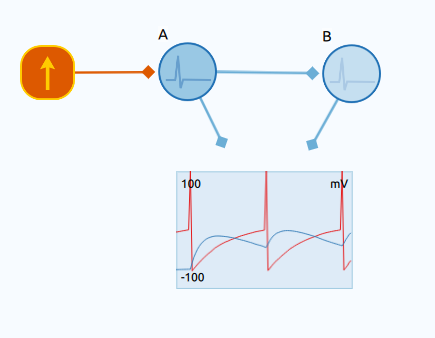
\includegraphics[width=8cm]{two_neurons.png}
\end{center}
\end{ExePart}

\begin{ExePart}
Note that the voltage trace from neuron B is very different from neuron A, because neuron A receives a steady current input, while neuron B receives the spikes from A. 

Using the default settings for both neurons, check that 75 mA is the smallest amount of Output Current from the current clamp that still allows neuron B to fire. Now, set the resting potential of both neurons to -70 mV, and attempt to find the minimum current output needed to induce spiking in neuron B.

\end{ExePart}
\end{Exercise}